\documentclass[11pt,a4paper]{report}
\usepackage[a4paper, left=20mm, right=20mm, top=30mm, bottom=20mm]{geometry}
\usepackage{amsmath,amsfonts,amssymb,amsthm,epsfig,epstopdf,titling,url,array,tkz-berge}
\usepackage[T2A,T1]{fontenc}
\usepackage[utf8]{inputenc}
\usepackage[russian]{babel}
\usepackage{xparse}
\usepackage[shortlabels]{enumitem}
\usepackage{float}
\usepackage{cancel}
\usepackage{multicol}
\usepackage{listings}

\usepackage{hyperref}
\hypersetup{
	colorlinks=true,
	linkcolor=blue,
	filecolor=magenta,      
	urlcolor=blue,
}
\def\E{\mathbb{E}}
\def\Var{\mathrm{Var}}
\def\cov{\mathrm{cov}}
\def\corr{\mathrm{corr}}
\def\salg{\mathcal{F}}
\def\P{\mathrm{P}}
\def\borel{\mathcal{B}}
\def\cantor{\mathcal{C}}

\def\eps{\varepsilon}
\def\phi{\varphi}
\def\Real{\mathbb{R}}
\def\Proj{\mathbb{P}}
\def\Hyper{\mathbb{H}}
\def\Integer{\mathbb{Z}}
\def\Natural{\mathbb{N}}
\def\Complex{\mathbb{C}}
\def\Rational{\mathbb{Q}}
\def \tr{\mbox{tr}}
\def \grad{\nabla}
\def \mse{\mbox{MSE}}
\def \etheta{\widehat{\theta}}

\def\le{\leqslant}
\def\ge{\geqslant}

\usepackage{eucal}
\usepackage{stackengine,graphicx,amssymb}
\stackMath
\newcommand\frightarrow{\scalebox{1}[.3]{$\rule[.45ex]{2ex}{1.5pt}%
		\kern-.2ex{\blacktriangleright}$}}
\newcommand\darrow[1][]{\mathrel{\stackon[1pt]{\stackanchor[1pt]{\frightarrow}{\frightarrow}}{\scriptstyle#1}}}

\newcommand\independent{\protect\mathpalette{\protect\independenT}{\perp}}
\def\independenT#1#2{\mathrel{\rlap{$#1#2$}\mkern2mu{#1#2}}}
\renewcommand{\thesection}{\arabic{section}}


\theoremstyle{definition}
\newtheorem{problem}{Задача}
\newtheorem*{uproblem}{Задача}

\theoremstyle{definition}
\newtheorem{theorem}{Теорема}[section]
\newtheorem{lemma}{Лемма}[section]
\newtheorem{preposition}{Утверждение}[section]
\newtheorem*{corollary}{Следствие} 
\theoremstyle{definition}
\newtheorem{definition}{Определение}[section]
\newtheorem{example}{Пример}[section]

\newcommand\mydots{\makebox[1em][c]{.\hfil.\hfil.}}
\renewcommand{\thesection}{\arabic{section}}

\usetikzlibrary{arrows.meta}
\usetikzlibrary{shapes.geometric}
\usepackage{etoolbox}

\title{Сложность вычислений\\\textit{<<Дерево Штейнера>>}}
\author{Иванов Вячеслав, группа 699}

\begin{document}
	\setlength{\parindent}{1cm}
	{\let\newpage\relax\maketitle}
	\tableofcontents
	\newpage 
	\section{Аннотация}
\textit{	Рассмотрена задача поиска дерева Штейнера — дерева минимального веса, соединяющего в том числе заданное фиксированное подмножество вершин, называемых терминальными — во взвешенном неориентированном графе. Доказана NP-полнота этой задачи и приведен 2-оптимальный алгоритм её решения. Произведен обзор приложений в таких задачах вычислительной биологии, как построение филогенетических деревьев, а также поиск метаболических путей и предсказание биомаркеров рака на основе сетей биологческих взаимодействий. }
	\section{Постановка задачи}
		 $G = (V, E)$ — неориентированный граф, $V_0 \subset V$ — непустое множество \textit{терминальных} вершин $\omega : E \to \Real^{+}$ — весовая функция. Требуется решить задачу оптимизации:
		\begin{align*}
			&\min_{T \subset G} \sum_{e \in E(T)} \omega(e)\\
			&\text{s.t.}\ 
			\begin{aligned}
				&T \text{ — дерево}\\
				&V_0 \subset V(T)			
			\end{aligned}
		\end{align*}
		Т.е. найти дерево минимального веса, покрывающее все терминальные вершины.\\
		В нетривиальных частных случаях задача имеет полиномиальный алгоритм решения:
		\begin{enumerate}
			\item $|V_0| = 2$: задача о кратчайшем пути между выделенными вершинами
			\item $V_0 = V$: задача о минимальном остовном дереве
		\end{enumerate}
		Алгоритмы поиска минимального остовного дерева, как будет показано далее, составляют основу 2-оптимального алгоритма поиска дерева Штейнера в метрическом случае.
	\section{Практическая значимость}
		Деревья Штейнера возникают в таком количестве практических задач, что на эту тему пишут \href{https://www.springer.com/gp/book/9781402000997}{целые книги}. Автору особенно приглянулись примеры из области его научных интересов:
	\subsection{Построение филогенетических деревьев}
	\begin{definition}
		\textit{Филогенетическое дерево} — корневое дерево, отражающее эволюционные связи и степень сходства между организмами. Построение таких деревьев — частая задача эволюционной биоинформатики.
	\end{definition}
	\begin{definition}
		\textit{Расстояние Левенштейна} или \textit{редакторское расстояние} $ L(s_1, s_2) $ — минимальная стоимость получения строки $s_2$ из строки $s_1$ применением операций вставки, удаления и замены символов друг на друга, каждая из которых имеет некоторую стоимость. 
	\end{definition}
	\begin{definition}
		\textit{Расстояние Хэмминга} $ H(s_1, s_2) $ определено для пар строк одинаковой длины $ n := |s_1| = |s_2| $ и выражается через число позиций, в которых $ s_1 $ и $ s_2 $ различаются: 
		$$
			H(s_1, s_2) = \sum_{i=1}^{n} \mathrm{I}\left (s_1^{(i)} \neq s_2^{(i)}\right )
		$$
	\end{definition} 
	\noindent В простейшей постановке из генома нескольких организмов взяты участки одинаковой длины. Каждая строка является терминальной вершиной, метрика — расстояние Хэмминга. Требуется построить дерево Штейнера. Утверждается, что оно является хорошим приближением реального филогенетического дерева, объединяющего эти организмы. В более общем случае последовательности могут иметь разную длины или состоять из нескольких несвязных частей. Тогда в качестве метрики используют расстояние Левенштейна, а на этапе предобработки данных выполняют \href{https://en.wikipedia.org/wiki/Sequence_alignment}{множественное выравнивание}, с помощью которого добиваются максимального подобия сравниваемых участков, взятых из разных организмов (что необходимо для получения биологически осмысленного результата).\\
	
	\noindent Больше про алгоритмы построения филогенетических деревьев можно прочитать в [UEL].
%	\clearpage
	\begin{figure}[!hbtp]
		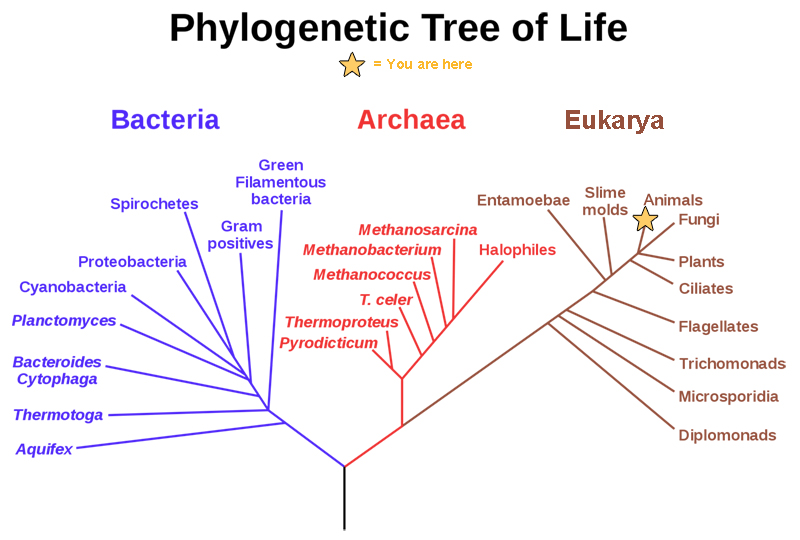
\includegraphics[width=\textwidth]{./img/phylogenetic_tree.jpg}
		\caption{\textit{Филогенетическое дерево, показывающее общее происхождение организмов из всех трёх доменов: Бактерии, Археи, Эукариоты.}}
	\end{figure}
	\clearpage
	\subsection{Анализ сетей биологических взаимодействий}
		\begin{figure}[!hbtp]
		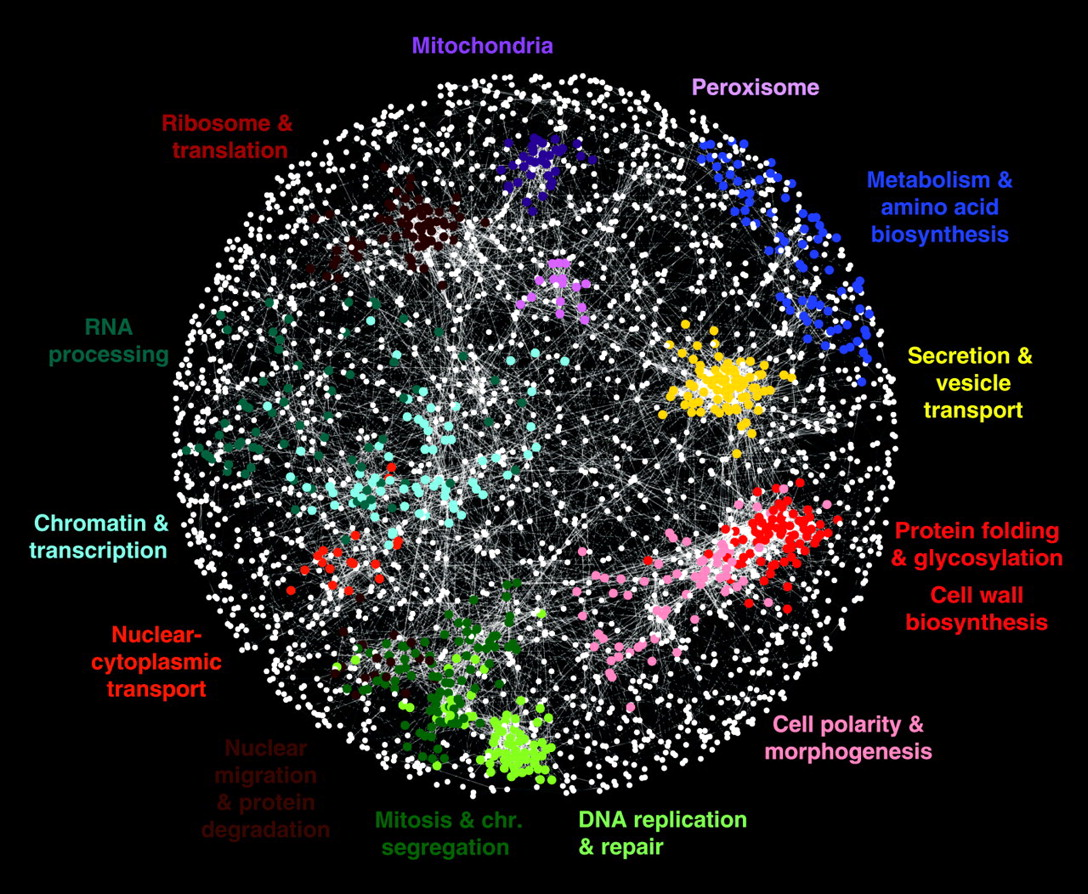
\includegraphics[width=\textwidth]{./img/yeast_interactome.jpg}
		\caption{\textit{Функциональные модули в геноме пекарских дрожжей Saccharomyces cerevisiae. \newline Источник — \href{http://thecellmap.org/}{http://thecellmap.org/}}}
	\end{figure}
	\begin{definition}
		\textit{Экспрессия генов} — процесс преобразования информации, закодированной в ДНК, в клеточные процессы и структуры. В контексте сетей чаще всего говорят про экспрессию матричной РНК (мРНК) и белков, синтезирующихся на её основе. Эти процессы называют \textit{транскрипцией} и \textit{трансляцией} соответственно.
	\end{definition}
	\begin{definition}
		\textit{Микрочип (microarray)} — устройство для измерения уровней экспрессии мРНК, представляющее собой кремниевую подложку с множеством ($\approx 10^3\ldots10^4$) выемок, каждая из которых содержит нить РНК, комплементарную мРНК, транскрибирующейся из исследуемого гена. Микрочипы заложили основу т.н. \textit{high-throughput NGS-методов}\footnote{NGS = Next Generation Sequencing, секвенирование нового поколения} — технологий, позволяющих одновременно измерять уровни экспрессии всех (или почти всех) генов в клетке.  
	\end{definition}
	\begin{definition}
		Если уровни экспрессии какого-то гена существенно различны в двух проведенных измерениях, то говорят, что имеет место \textit{дифференциальная экспрессия генов (differential gene expression)}. Анализ дифференциальной экспрессии проводят для того, чтобы лучше понять течение заболевания или обнаружить, какие именно гены влияют на наблюдаемые признаки.
	\end{definition}
	\begin{definition}
		\textit{Интерактом} — ориентированный граф с петлями и кратными рёбрами, кодирующий все взаимодействия между молекулами в клетке. В нём выделяют такие важные подграфы, как:
		\begin{itemize}
			\item Граф белок-белковых взаимодействий, он же \textit{протеом} (чаще всего имеют в виду его).
			\item Метаболическая сеть (преобразования молекул друг в друга под воздействием энзимов)
		\end{itemize}
	\end{definition}
	\noindent Расцвет high-throughput методов привёл к тому, что современная геномика генерирует больше данных, чем астрономия и интернет. Человечество получило возможность построить более-менее полные интерактомы основных модельных организмов и интегрировать это знание в анализ дифференциальной экспрессии генов.\\
	
	\noindent Типичная задача, в контексте которой при этом возникает дерево Штейнера, выглядит так: в некоторой группе генов, играющих роль множества терминальных вершин $V_0$, обнаружена существенная дифференциальная экспрессия, и есть подозрение, что тому есть общая причина в виде конкретных полиморфизмов\footnote{Полиморфизм — стабильный вариант гена, обычно отличающийся в одном нуклетоиде}, метаболических путей и т.д.\\
	
	\noindent В качестве конкретного примера можно привести работу [BMC]. Авторы пишут, что гены, мутации в которых приводят к прогрессии онкозаболеваний, не всегда можно найти при помощи анализа дифференциальной экспрессии. Тем не менее, довольно часто они оказывают скрытое влияние на гены с ярко выраженной картиной дифференциальной экспрессии — так называемые биомаркеры рака, — входя с ними в одни и те же метаболические пути. К сожалению, для большинства генов в геноме человека неизвестно, в каких метаболических путях они участвуют. Тем не менее, сеть взаимодействий между генами довольно хорошо изучена. Более того, есть алгоритмы предсказания новых взаимодействий на основе уже имеющихся данных. Авторы демонстрируют, что поиск дерева Штейнера, соединяющего гены из некоторого поднабора достоверно известных биомаркеров, позволяет найти остальные и сформировать список кандидатов для дальнейшего исследования. \\
	 
	\noindent Степень уверенности в том, что для данного гена имеет место дифференциальная экспрессия, обычно выражается в терминах p-значений.\footnote{Конкретные способы подсчёта этих p-значений — отдельная сложная тема, выходящая за рамки данной работы} Для проверки гипотез о связях между такими генами в графе взаимодействий вводится весовая функция по следующему правилу: если хотя бы один из концов ребра не является терминальной вершиной, то весом будет степень уверенности в достоверности этого ребра\footnote{Большая проблема подходов, использующих интерактом, в том, что все рёбра в нём отражают реальность только лишь с некоторой степенью уверенности. Существенная часть рёбер была предсказана на компьютере и не имеет экспериментального подтверждения, что вызывает критику в научном сообществе.}, иначе учитывают также и вклад корреляции между их p-значениями. Т.е. дерево Штейнера должно максимизировать правдоподобие составляющих его рёбер, причём чем более выражена корреляция между признаками, тем б\textbf{о}льший вклад даёт ребро между ними. Построенное дерево позволяет выявить гены или метаболиты, которые оказывают наибольшее влияние на экспрессию генов из $V_0$, что позволяет выявить скрытые биологические закономерности, недоступные или неочевидные для непосредственного наблюдения.\\
	
	\noindent Задача поиска дерева Штейнера в биологических сетях имеет свои особенности в связи как со статистической природой рёбер в таких сетях, так и с их структурой — большая часть таких сетей являются безмасштабными  (\href{https://en.wikipedia.org/wiki/Scale-free_network}{scale-free}). Вычислительные эксперименты [UT] показывают, что размеры таких графов, равно как и множества $V_0$, можно значительно (в разы) сократить, убрав из рассмотрения вершины, которые точно не войдут в дерево Штейнера, что позволяет подсчитать точный ответ (с помощью алгоритма Дрейфуса-Вагнера, как в [UT]).\\
	
	\noindent Больше про различные подходы к предобработке данных при поиске дерева Штейнера и о приложениях последнего в анализе биологических сетей можно прочитать в [UT]. Автор данной работы пока не использовал деревья Штейнера в своей научной практике, но заинтересован.
	\subsection{Краткий обзор других приложений}
	С изобилием вариаций задачи о дереве Штейнера можно ознакомиться в обзоре [UB].
	\section{Доказательство NP-полноты задачи}
	\begin{theorem}
		$$ \{ (G, k)\ |\ \text{ в неориентированном графе $ G $ есть дерево Штейнера весом не более чем } k \in \Integer   \} \in \mathrm{NPC} $$
	\end{theorem}
	\begin{proof}[Доказательство $ \text{[EPFL]} $]$  $
		\begin{enumerate}
			\item \textbf{STEINER-TREE $\in$ NP}: 
				Сертификат должен проверять, что поданный ему на вход подграф $T$ является деревом, содержит все терминальные вершины и имеет вес $\le k$, причём вторая и третья подзадачи тривиальны. Согласно одному из эквивалентных определений дерева, достаточно проверить связность $T$ и то, что $|E(T)| = |V(T)| - 1$, для чего достаточно обхода в глубину. Т.е. полиномиальный сертификат существует и STEINER-TREE $\in$ NP.
			\item \textbf{VERTEX-COVER $\le_{p}$ STEINER-TREE}: Полиномиальное сведение устроено так:
			\begin{enumerate}
				\item Дополним $G = (V, E)$ до полного графа, после чего произведём подразделение всех исходных рёбер. Множество добавленных при этом вершин обозначим через $ W $, а полученный в результате граф — через $ G' := (V', E') $. Всем рёбрам назначим единичные веса, а весовую функцию будем как и раньше обозначать через $ \omega $.
				\begin{figure}[!hbtp]
				\centering
					\begin{tikzpicture}
					\pgfmathsetmacro{\n}{4}
					\pgfmathsetmacro{\rotangle}{360 / (2 * \n)}
					\pgfmathsetmacro{\disttoside}{5.65}
					\node[draw=none,minimum size=8cm,regular polygon,regular polygon sides=\n] (poly) {};
					\begin{scope}[>={Stealth[black]},
						every node/.style={fill=white,circle},
						every edge/.style={draw=blue,thick,dashed}]
						\foreach \x in {1,2,...,\n} {
							\path[-] (0, 0) edge node {$1$} (poly.corner \x);
						}
					\end{scope}
					\node[draw=none,minimum size=\disttoside cm,regular polygon,regular polygon sides=\n, shape border rotate = \rotangle] (polyrot) {};
					\begin{scope}[>={Stealth[black]},
						every node/.style={fill=white,circle},
						every edge/.style={draw=black,thick}]
						\foreach \x in {1,2,...,\n} {
							\pgfmathtruncatemacro{\cur}{\x};
							\pgfmathtruncatemacro{\next}{max(1, Mod(\cur + 1, \n + 1)};
							\path[-] (poly.corner \cur) edge node {$1$} (polyrot.corner \cur);
							\path[-] (polyrot.corner \cur) edge node {$1$} (poly.corner \next);
						}
					\end{scope}
					\begin{scope}[every node/.style={circle,thick,draw}]
						\foreach \idx in {1,2,...,\n} {
							\fill[red] (poly.corner \idx) circle[radius=4pt];
						}
					\end{scope}
					\begin{scope}[every node/.style={circle,thick,draw}]
						\foreach \idx in {1,2,...,\n} {
							\fill[cyan] (polyrot.corner \idx) circle[radius=4pt];
						}
					\end{scope}
					\end{tikzpicture}
					\caption{\textit{Пример конструкции: красные вершины — $ V $, голубые — $W$, штрихпунктирные рёбра добавлены при дополнении до полного графа, сплошные были изначально. Все веса единичные. }}
				\end{figure}
				\item Если теперь в качестве множества терминальных вершин $ V_0' $ взять $ W $, то в $G'$ есть дерево Штейнера веса $ \le |E| + k - 1 \iff $ в $G$ есть вершинное покрытие мощности $\le k$.
			\end{enumerate}
			\begin{proof}$  $
				\begin{itemize}
					\item $ \underline{\implies} $: Пусть $T$ — дерево Штейнера для $V_0'$ в $G'$, тогда $C := V(T) \setminus V_0'$ — вершинное покрытие в $G$. Действительно, $ C \subset V $ и накрывает каждое ребро $e \in E$ по построению, ведь терминальные вершины появились при подразделении рёбер из $E$. Также:
					$$ |C| = |V(T)| - |V_0'| = \omega(T) + 1 - |V_0'| \le (|E| + k - 1) + 1 - |V_0'| = k,$$ т.к. $|E| = |V_0'|$ по построению. 
					\item $ \underline{\impliedby} $:  Пусть $C \subset V$ — вершинное покрытие, $|C| \le k$, а $T$ — дерево на вершинах $C$ в $G'$.\footnote{Такое дерево всегда существует, т.к. $V^2 \subset V(G')$.} Хотим, чтобы это дерево покрывало множество терминальных вершин. Чтобы гарантировать, что $V_0' \subset V(T)$, расширим $T$, если это необходимо: для каждой вершины $v_0' \in V_0' \setminus V(T)$ добавим к $T$ ребро $(v_0', c)$, где $c \in C$ — вершина покрытия, накрывающая ребро, подразделением которого получена вершина $v_0'$. Полученный граф содержит $\le |E| + |C| - 1 \le |E| + k - 1$ рёбер. Если при добавлении рёбер в $T$ образовались циклы, их можно раскрыть, уменьшив суммарный вес. По завершении получим дерево Штейнера веса $\le |E| + k - 1$ для $V_0'$ в $G'$.
				\end{itemize} 
			\end{proof}
			Все шаги построения $G'$ полиномиальны: добавляется $O(|V|^2)$ рёбер и вершин. Для восстановления вершинного покрытия по дереву Штейнера в $G'$ нужно брать разность множеств — $O(|V|^2)$ операций, а в обратную сторону нужно перебрать $V_0'$ и исходящие из него рёбра (не более двух на каждую вершину) — тоже $O(|V|^2)$ операций.
		\end{enumerate}
	\end{proof}
	\section{Сведение к метрическому случаю}
		Часто хочется потребовать, чтобы для весовой функции выполнялось правило треугольника:
		$$
			\omega(x, y) \le \omega(x, z) + \omega(z, y),		
		$$
		причём она должна быть определена на $V^2$. Такая весовая функция играет роль метрики на множестве вершин и становится проще для восприятия. В таком случае говорят о поиске \textit{метрического} дерева Штейнера, и именно такой вид задачи был исторически первым.
		\begin{preposition}$  $
			\begin{enumerate}
				\item Существует полиномиальное сведение задачи о дереве Штейнера к метрическому случаю.
				\item Оптимальные ответы к обеим задачам совпадают.
			\end{enumerate}
		\end{preposition}
		\begin{proof}
			Предложенная конструкция основана на понятии \textit{метрического замыкания}:
			\begin{definition}
				Пусть $ G = (V, E, \omega) $ — неориентированный взвешенный граф, $d: V^2 \to \Real^{+} $ — функция расстояния, сопоставляющая паре вершин длину кратчайшего пути между ними. Тогда граф $G' = (V', E')$ называется \textit{метрическим замыканием} графа $G$:
				$$
					G' = (V, E', d),\ E' = \{ (u, v)\ |\ u, v \in V,\ u \neq v \}
				$$
				Полученный граф является метрическим, т.к. для $d$ выполнено правило треугольника: если $ d(x, y) > d(x, z) + d(z, y) $, то путь $x \to y$ можно было бы прорелаксировать конкатенацией путей $x \to z$ и $z \to y$, что противоречит определению $d(x, y)$ как длины \textit{кратчайшего} пути $x \to y$.\\
				Построить метрическое замыкание можно за $O(|V|^3)$ алгоритмом Флойда-Уоршелла. 
			\end{definition}
			\noindent Пусть $T, T'$ — деревья Штейнера для $V_0$ в $ G $ и $ G' $ соответственно. Докажем, что $\omega(T) = d(T')$. Очевидно, что $ d(T') \le \omega(T) $, т.к. переход к кратчайшим путям не ухудшает ответ. Более того, каждое ребро в $T'$ можно <<разжать>> в тот кратчайший путь, из которого он был получен, после чего выбрать в полученном графе минимальное остовное дерево $T''$. $\omega(T'') \le d(T')$, т.к. теперь каждое ребро встречается ровно один раз, а ранее могло вносить свой вклад одновременно в несколько кратчайших путей. Но $T''$ по построению — дерево Штейнера для $V_0$ в $G$! Следовательно, $ \omega(T) = \omega(T'') \le d(T') \le \omega(T)$, т.е. $\omega(T) = d(T')$.
 		\end{proof}
	\section{2-оптимальный алгоритм}
	\begin{theorem}$  $\\
		Существует 2-оптимальный алгоритм, основанный на сведении задачи к метрическому случаю:
		\begin{enumerate}
			\item Построить метрическое замыкание $G' = (V, E', d)$ графа $G$.
			\item Выделить $H'$ — подграф в $G'$, индуцированный терминальными вершинами из $V_0$. 
			\item Построить минимальное остовное дерево $T_{\mathrm{MST}}$ в $H'$.
			\item Вернуть в качестве ответа дерево в $G$, восстановленное из $T_{\mathrm{MST}} $ заменой рёбер между вершинами на соответствующие кратчайшие пути в графе $G$.
		\end{enumerate}
	\end{theorem}
	\begin{proof}[Доказательство $ \text{[St]} $]$  $\\
		Пусть $T_{S}$ — дерево Штейнера для $V_0$ в $G'$, $ |V_0| = k+1 $.\\
		Выпишем вершины $T_{S}$ в порядке обхода в глубину. Будем добавлять вершину в список и при каждом выходе из неё по исходящему ребру, и по возвращению из рекурсивного вызова. Получим массив, называемый эйлеровым обходом дерева $T_{S}$:
		$$
			u_0, u_1, \ldots, u_m = u_0
		$$ 
		Такой обход задаёт Эйлеров цикл, поскольку в алгоритм обхода запрещает проходить по одному ребру дважды. Значит:
		$$ 
			\sum_{i=0}^{m-1} d(u_i, u_{i+1}) = 2 \cdot d(T_{S})
		$$
		Если исключить из рассмотрения все нетерминальные вершины и оставить только первое вхождение всех терминальных, не меняя порядок вхождения вершин, то получим путь\footnote{Поскольку мы работаем с метрическим замыканием, рёбра $(v_{i}, v_{i+1})$ в графе $G'$ гарантированно есть.}:
		$$
			v_0, v_1, \ldots, v_k
		$$
		содержащий все терминальные вершины (т.к. изначально это был обход связного графа $G'$).\\ 
		По неравенству треугольника:
		$$
			d(v_i, v_{i+1}) \le \sum_{j=1}^{t} d(u_{i_j}, u_{i_{j+1}})
		$$
		Здесь $ u_{i_{1}},\ldots, u_{i_{t+1}} $ — подотрезок в эйлеровом обходе, т.е. $v_i = u_{i_{1}}, v_{i+1} = u_{i_{t+1}}$, причём подотрезки для каждой пары $ (v_{i}, v_{i+1}) $ не пересекаются, т.к. в исходном эйлеровом обходе \textit{первые} вхождения этих вершин встречаются именно в таком порядке.\\
		Поскольку $v_0, \ldots, v_k$ — путь, это также дерево. Более того, в силу того, как задана весовая функция, это ещё и минимальное остовное дерево $T_{\mathrm{MST}}$ в $H'$, причём:
		\begin{gather*}
			d(T_{\mathrm{MST}}) = \sum_{i=0}^{k-1} d(v_{i}, v_{i+1}) \le \sum_{i=0}^{m-1} d(u_i, u_{i+1}) = 2 \cdot d(T_{S})\\
			1 \le \frac{d(T_{\mathrm{MST}})}{d(T_{S})} \le 2
		\end{gather*}
		По \textit{утверждению 3.1.}, по нему восстанавливается дерево Штейнера в $G$.
	\end{proof}
	\begin{figure}[!hbtp]
	\centering
	\begin{tikzpicture}
		\pgfmathsetmacro{\n}{7}
		\node[draw=none,minimum size=6cm,regular     polygon,regular polygon sides=\n] (poly) {};
		\begin{scope}[>={Stealth[black]},
			every node/.style={fill=white,circle},
			every edge/.style={draw=blue,thick}]
			 \foreach \x in {1,2,...,\n} {
		 		\path[-] (0, 0) edge node {$1$} (poly.corner \x);
			 }
		\end{scope}
		\begin{scope}[>={Stealth[black]},
			every node/.style={fill=white,circle},
			every edge/.style={draw=red,thick}]
			\foreach \x in {1,2,...,\n} {
				\pgfmathtruncatemacro{\cur}{\x};
				\pgfmathtruncatemacro{\next}{max(1, Mod(\cur + 1, \n + 1)};
				\path[-] (poly.corner \cur) edge node {$2$} (poly.corner \next);
			}
		\end{scope}
		\begin{scope}[>={Stealth[black]},
			every node/.style={fill=white,circle},
			every edge/.style={draw=black,thick}]
				\path[-] (poly.corner \n) edge node {$2$} (poly.corner 1);
		\end{scope}
		\begin{scope}[every node/.style={circle,thick,draw}]
			\fill[black] (0, 0) circle[radius=4pt];
			\foreach \x in {1,2,...,\n} {
				\fill[red] (poly.corner \x) circle[radius=4pt];
			}
		\end{scope}
	\end{tikzpicture}
		\caption{Пример графа, на котором оценка достигается (в пределе). Терминальные вершины выделены красным. Реальное дерево Штейнера $ T_{S} $ выделено синим, а $ T_{\mathrm{MST}} $, построенное алгоритмом, — красным. Если внешний цикл имеет вид $n$-угольника, то верно, что $ \frac{d(T_{\mathrm{MST}})}{d(T_{S})} = \frac{2n-2}{n} = 2 - \frac{2}{n} \to 2 $. } 
	\end{figure}
	\section{Реализация}
	\subsection{Асимптотика работы алгоритма и ограничения по его применению}
	\begin{enumerate}
		\item Алгоритм Флойда-Уоршелла поиска кратчайших путей между всеми парами вершин: $\Theta(|V|^3)$ операций, $ \Theta(|V|^2) $ памяти на хранение матрицы расстояний. 
		\item Алгоритм Краскала поиска минимального остовного дерева с помощью системы непересекающихся множеств: $O(|E| \log |V|)$ операций, $ \Theta(|V|) $ памяти. 
	\end{enumerate}
	Т.к. метрическое замыкание делает граф полным, итого имеем $ \Theta(|V|^3) $ операций и $\Theta(|V|^2)$ памяти. Следовательно, алгоритм оправданно применять при $ |V| \le 1000 $, что является существенным недостатком предложенного подхода.\\
	
	\noindent Также стоит отметить, что алгоритмы Флойда-Уоршелла и Краскала по своей природе последовательные, в связи с чем воспользоваться преимуществами вычислительного кластера МФТИ, к которому автор имеет авторизованный доступ, не представляется возможным при таком подходе.\\
	
	\noindent Более того, алгоритм Флойда-Уоршелла хорош тем, что не совершает больших прыжков по памяти при хранении матрицы кратчайших расстояний в виде последовательно расположенной в памяти двумерной таблицы, что уменьшает число промахов по кэшу процессора и оказывает положительный эффект на скорость работы алгоритма по сравнению с параллельными запусками алгоритмов поиска кратчайших путей из данной вершины во все остальные (в духе алгоритма Дейкстры) при малых $|V|$.\\
	
	\noindent Тем не менее, при $|V| \ge 10^3$ не лишено смысла хранить исходную матрицу расстояний в базе данных (на жёстком диске или распределённо) и действительно выполнять параллельные запуски, скажем, алгоритма Дейкстры на доступных процессорах для параллельного подсчёта матрицы кратчайших расстояний. Эта неасимптотическая оптимизация делает возможной обработку существенно б\textbf{о}льших графов, чем было заявлено изначально, т.к. это типичная map-reduce задача, что с точки зрения автора является довольно дешёвой в реализации, но полезной идеей, пусть и выходящей за рамки требований поставленной учебной задачи. 
	
	\subsection{Использованные технологии}
			Для работы с графами в Python была использована библиотека \href{https://graph-tool.skewed.de/static/doc/topology.html#graph_tool.topology.shortest_distance}{graph-tool}. По опыту автора, альтернативы в лице \href{https://networkx.github.io/}{networkx} и \href{https://igraph.org/python/}{igraph} имеют слишком много нетривиальных недостатков: networkx написана на Pure Python, из-за чего производительность становится неприемлемой уже на маленьких графах, а разработка Python-API для написанной на C библиотеки igraph уже больше года как приостановлена, а по состоянию на данный момент пользоваться ей очень уж неудобно по причинам, расписывать которые слишком долго для того, чтобы приводить их здесь. Справедливости ради, R-API для igraph гораздо лучше, но Python для меня предпочтительнее.
	\subsection{Проверка корректности}
		Тесты разделены на несколько групп:
		\begin{enumerate}
			\item Маленькие ($|V| \le 20$) случайные графы в модели Эрдеша-Реньи, реальное дерево Штейнера в которых ищется полным перебором (возможно, с некоторыми эвристиками).
			\item Некоторые последовательности графов с известным точным ответом.
		\end{enumerate}
		Написание тестов, иллюстрирующих биологические приложения алгоритма, затруднительно в силу необходимости знаний предметной области для интерпретации результатов. Заинтересованный читатель может ознакомиться с ними в [BMC].
	\subsection{Результаты}
	Ознакомиться с реализацией можно \href{https://nbviewer.jupyter.org/github/ivanov-v-v/SteinerTree/blob/master/notebooks/SteinerTree.ipynb}{по ссылке}.\\
	Поскольку построение метрического замыкания — ключевой этап алгоритма, оно же ограничивает его применимость. Даже при параллельном поиске кратчайших путей алгоритмом Дейкстры или его модификациями и с хранением графа и матрицы расстояний в разделяемой памяти, не удастся добиться асимпотики лучше, чем $O(|V|^3)$ по времени и $O(|V|^2)$ по памяти, в связи с чем использовать алгоритм при $|V| \ge 10^4 $ нерационально и непрактично.\\
	Тем не менее, алгоритм прост в реализации, а его показатель аппроксимации отличается от оптимального на данный момент показателя в $\approx 1.55$ [CSV] всего на $\approx 0.45$.
	\section{Список литературы}
	\renewcommand\bibname{}
	\patchcmd{\thebibliography}{\chapter*}{\section*}{}{}
	\vspace*{-1cm}
	\begin{thebibliography}{}
		\bibitem{EPFL}[EPFL] \href{https://dcg.epfl.ch/wp-content/uploads/2018/10/9-NPHardness.pdf}{Chair of Combinatorial Geometry, EPFL — Lectures on Computational Complexity Theory}
		\bibitem{St}[St] \href{https://people.eecs.berkeley.edu/~luca/cs261/lecture02.pdf}{Luca Trevisan; Stanford University — "Approximating the Metric Steiner Tree Problem"}
		\bibitem{UB}[UB]
		 \href{http://theory.cs.uni-bonn.de/info5/steinerkompendium/netcompendium.pdf}{M.Hauptmann, M.Karpinski; Universität Bonn - A Compendium On Steiner Tree Problems}
		\bibitem{UT}[UT] \href{https://fpt.akt.tu-berlin.de/publications/steiner-tree-betzler06.pdf}{N. Betzler; Universität Tübingen — "Steiner Tree Problems in the Analysis of Biological Networks"}
		\bibitem{UEL}[UEL] \href{http://web.cs.elte.hu/~berkri/Theses/Biro.pdf }{Regina Krisztina Bíró, Eötvös Loránd University — "Constructing Phylogenetic Trees"}
		\bibitem{BMC}[BMC] \href{https://www.ncbi.nlm.nih.gov/pmc/articles/PMC3481447/}{Md Jamiul Jahid, Jianhua Ruan; BMC Genomics. 2012; 13(Suppl 6): S8. — "A Steiner tree-based method for biomarker discovery and classification in breast cancer metastasis"}
		\bibitem{CSV}[CSV] \href{https://www.cs.virginia.edu/~robins/papers/soda2000_camera.pdf}{Gabriel Robinsy, Alexander Zelikovsky; — "Improved Steiner Tree Approximation in Graphs"}
	\end{thebibliography}
\end{document}     